

\documentclass{book}

\usepackage{cite}
\author{Author Names}
\title{Maths Book Example using Latex}
\usepackage{mathtools}
\usepackage[table]{xcolor}
\usepackage{parskip}
\usepackage{xcolor}

%\usepackage{amssymb}
%\usepackage{amsthm}


\usepackage{tikz}
\begin{document}

\maketitle
\tableofcontents

\chapter{One}
\section{First section: Maths}

Grec Letters: 
\begin{equation}
%%   \alpha, \Alpha, \beta, \Beta, \gamma, \Gamma, \pi, \Pi, \phi, \varphi, \mu, \Phi 
   \alpha \text{and} \beta
\end{equation}

\begin{equation} \label{eu_eqn}
e^{\pi i} + 1 = 0
\end{equation}
 
The beautiful equation \ref{eu_eqn} is known as the Euler 
equation.


Square root:
\begin{equation}
  \sqrt[n]{1+x+x^2+x^3+\dots+x^n} 
\end{equation}

Sum:
\begin{equation}
  \displaystyle\sum_{i=1}^{10} t_i 
\end{equation}

Formulas:
\begin{equation}
   \cos (2\theta) = \cos^2 \theta - \sin^2 \theta  
\end{equation}

Limits: 
\begin{equation}
   \lim\limits_{x \to \infty} \exp(-x) = 0  
\end{equation}


Delimiter:
\begin{equation}
  \left.\frac{x^3}{3}\right|_0^1 
\end{equation}


Equation: 
\begin{equation}
  x = a_0 + \cfrac{1}{a_1 
          + \cfrac{1}{a_2 
          + \cfrac{1}{a_3 + \cfrac{1}{a_4} } } }
\end{equation}





\section{Second section: Tables}
\begin{tabular}{ | l | c | r  | }
  \hline			
   \cellcolor{blue!25}coloured &  \cellcolor{blue!25}coloured &   \cellcolor{blue!25}coloured     \\
  \hline			
  1 & 2 & 3 \\
  \hline			
  3 & 4 & 6 \\
  \hline  
\end{tabular}

\vspace{1cm}

\begin{tabular}{ l c r }
  1 & 2 & 3 \\
  4 & 5 & 6 \\
  7 & 8 & 9 \\
\end{tabular}





\vspace{1cm}


\begin{tabular}{ l | c | r }
  \hline			
  1 & 2 & 3 \\
  4 & 5 & 6 \\
  7 & 8 & 9 \\
  \hline  
\end{tabular}



\vspace{1cm}

With width specified:
\begin{center}
    \begin{tabular}{ | l | l | l | p{5cm} |}
    \hline
    Day & Min Temp & Max Temp & Summary \\ \hline
    Monday & 11C & 22C & A clear day with lots of sunshine.  
    However, the strong breeze will bring down the temperatures. \\ \hline
    Tuesday & 9C & 19C & Cloudy with rain, across many northern regions. Clear spells 
    across most of Scotland and Northern Ireland, 
    but rain reaching the far northwest. \\ \hline
    Wednesday & 10C & 21C & Rain will still linger for the morning. 
    Conditions will improve by early afternoon and continue 
    throughout the evening. \\
    \hline
    \end{tabular}
\end{center}



\section{Third section:  Matrix}
This will display a first matrix into an equation:
\begin{equation}
 \begin{matrix}
  a & b & c \\
  d & e & f \\
  g & h & i
 \end{matrix}
\end{equation}


\begin{equation}
A_{m,n} = 
 \begin{pmatrix}
  a_{1,1} & a_{1,2} & \cdots & a_{1,n} \\
  a_{2,1} & a_{2,2} & \cdots & a_{2,n} \\
  \vdots  & \vdots  & \ddots & \vdots  \\
  a_{m,1} & a_{m,2} & \cdots & a_{m,n} 
 \end{pmatrix}
\end{equation}


\begin{equation}
M = \begin{bmatrix}
       \frac{5}{6} & \frac{1}{6} & 0           \\[0.3em]
       \frac{5}{6} & 0           & \frac{1}{6} \\[0.3em]
       0           & \frac{5}{6} & \frac{1}{6}
     \end{bmatrix}
\end{equation}



\section{Fourth Section: Cite}
Lorem ipsum dolor sit amet, consectetur adipiscing elit, sed do eiusmod tempor incididunt ut labore et dolore magna aliqua. Ut enim ad minim veniam, quis nostrud exercitation ullamco laboris nisi ut aliquip ex ea commodo consequat. Duis aute irure dolor in reprehenderit in voluptate velit esse cillum dolore eu fugiat nulla pariatur. Excepteur sint occaecat cupidatat non proident, sunt in culpa qui officia deserunt mollit anim id est laborum.
This text will cite some references \cite{refpub1549567168A019, refpub1549567168A020,refpub1549567168A021}.
This text will cite some references \cite{refpub1549567168A019, refpub1549567168A020,refpub1549567168A021}.
This text will cite some references \cite{refpub1549567168A019, refpub1549567168A020,refpub1549567168A021}.
This text will cite some references \cite{refpub1549567168A019, refpub1549567168A020,refpub1549567168A021}.
This text will cite some references \cite{refpub1549567168A019, refpub1549567168A020,refpub1549567168A021}.
This text will cite some references \cite{refpub1549567168A019, refpub1549567168A020,refpub1549567168A021}.
This text will cite some references \cite{refpub1549567168A019, refpub1549567168A020,refpub1549567168A021}.
This text will cite some references \cite{refpub1549567168A019, refpub1549567168A020,refpub1549567168A021}.
This text will cite some references \cite{refpub1549567168A019, refpub1549567168A020,refpub1549567168A021}.
This text will cite some references \cite{refpub1549567168A019, refpub1549567168A020,refpub1549567168A021}.
This text will cite some references \cite{refpub1549567168A019, refpub1549567168A020,refpub1549567168A021}.
Lorem ipsum dolor sit amet, consectetur adipiscing elit, sed do eiusmod tempor incididunt ut labore et dolore magna aliqua. Ut enim ad minim veniam, quis nostrud exercitation ullamco laboris nisi ut aliquip ex ea commodo consequat. Duis aute irure dolor in reprehenderit in voluptate velit esse cillum dolore eu fugiat nulla pariatur. Excepteur sint occaecat cupidatat non proident, sunt in culpa qui officia deserunt mollit anim id est laborum.


\section{Fifth Section: Figures}
Lorem ipsum dolor sit amet, consectetur adipiscing elit, sed do eiusmod tempor incididunt ut labore et dolore magna aliqua. Ut enim ad minim veniam, quis nostrud exercitation ullamco laboris nisi ut aliquip ex ea commodo consequat. Duis aute irure dolor in reprehenderit in voluptate velit esse cillum dolore eu fugiat nulla pariatur. Excepteur sint occaecat cupidatat non proident, sunt in culpa qui officia deserunt mollit anim id est laborum.
This text will describe the first figure below which is Fig. \ref{fig:figtikz01}.
This text will describe the second figure below which is Fig. \ref{fig:figtikz02}.

\begin{figure}[h!]
\begin{center}
    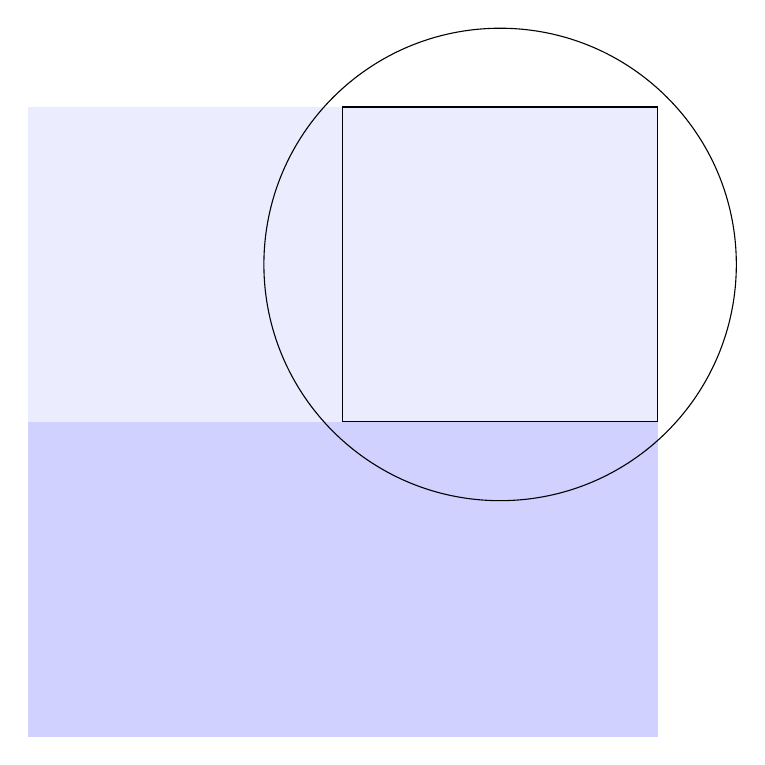
\begin{tikzpicture}
    % define coordinates
    \coordinate (O) at (0,0) ;
    \coordinate (A) at (0,4) ;
    \coordinate (B) at (0,-4) ;
    % media
    \fill[blue!25!,opacity=.3] (-4,0) rectangle (4,4);
    \fill[blue!60!,opacity=.3] (-4,0) rectangle (4,-4);
    \draw (2,2) circle (3cm);
    \draw (0,0) -- (4,0) -- (4,4) -- (0,4) -- (0,0);
    \end{tikzpicture}
\caption{The first figure using tikz}
\label{fig:figtikz01}
\end{center}
\end{figure}

Lorem ipsum dolor sit amet, consectetur adipiscing elit, sed do eiusmod tempor incididunt ut labore et dolore magna aliqua. Ut enim ad minim veniam, quis nostrud exercitation ullamco laboris nisi ut aliquip ex ea commodo consequat. Duis aute irure dolor in reprehenderit in voluptate velit esse cillum dolore eu fugiat nulla pariatur. Excepteur sint occaecat cupidatat non proident, sunt in culpa qui officia deserunt mollit anim id est laborum.
This text will cite some references \cite{refpub1549567168A019}.
Lorem ipsum dolor sit amet, consectetur adipiscing elit, sed do eiusmod tempor incididunt ut labore et dolore magna aliqua. Ut enim ad minim veniam, quis nostrud exercitation ullamco laboris nisi ut aliquip ex ea commodo consequat. Duis aute irure dolor in reprehenderit in voluptate velit esse cillum dolore eu fugiat nulla pariatur. Excepteur sint occaecat cupidatat non proident, sunt in culpa qui officia deserunt mollit anim id est laborum.
This text will cite some references \cite{refpub1549567168A020,refpub1549567168A021}.
Lorem ipsum dolor sit amet, consectetur adipiscing elit, sed do eiusmod tempor incididunt ut labore et dolore magna aliqua. Ut enim ad minim veniam, quis nostrud exercitation ullamco laboris nisi ut aliquip ex ea commodo consequat. Duis aute irure dolor in reprehenderit in voluptate velit esse cillum dolore eu fugiat nulla pariatur. Excepteur sint occaecat cupidatat non proident, sunt in culpa qui officia deserunt mollit anim id est laborum.
This text will cite some references \cite{refpub1549567168A021}.



\begin{figure}[h!]
\begin{center}
    \begin{tikzpicture}
    % define coordinates
    \coordinate (O) at (0,0) ;
    \coordinate (A) at (0,4) ;
    \coordinate (B) at (0,-4) ;
    % media
    \draw (2,0) -- (8,0) -- (4,8) -- (0,7) -- (0,0);
    \end{tikzpicture}
\caption{The second simple figure using tikz}
\label{fig:figtikz02}
\end{center}
\end{figure}

\bibliography{mybib}{}
\bibliographystyle{ieeetr}
\end{document}

